\chapter{Learning BN}
\label{cha:learning_BN} As explained in Section \ref{sec::practicalSuggestions} when
building a Bayesian Network it is crucial to collaborate with a domain expert in
order to follow as much as possible causality relationships among variables. At
the beginning of this section we assume that the structure of the model is given.\\
We are given a dataset (training set) of examples
$\mathcal{D}= \{\pmb{x}(1), ..., \pmb{x}(N)\}$. Each example $\pmb{x}(i)$ is a configuration
for \textit{all} (complete data) or \textit{some} (incomplete data) variables in
the model (which is the Bayesian network).
\newline

\textbf{Task:} we need to estimate the parameters of the model (conditional probability
distributions) from the data.
\newline

The simplest approach consists of learning the parameters maximizing the
likelihood of the data:
\[
	{\pmb{\theta}}^{\mathit{max}}={\mathit{argmax}}_{\pmb{\theta}}p(\mathcal{D}|\pmb
	{\theta}) = \mathit{argmax}_{\pmb{\theta}}\mathcal{L}(\mathcal{D}, \pmb{\theta}
	)
\]
As we have discussed in Section \ref{par:maximum_likelyhood_estim} this method is
referred to as \textit{Maximum likelihood estimation}. In the formula $\mathcal{L}
(\mathcal{D}, \pmb{\theta})$ is the likelihood function to maximize with respect
to the parameters.
\newline

Probabilistic graphical models allow to graphically represent relationships among
examples and parameters. Suppose we have three variables linked together with a
tail-to-tail configuration as illustrated in Figure
\ref{fig:tailToTailLearningBN}.

\begin{figure}[H]
	\centering
	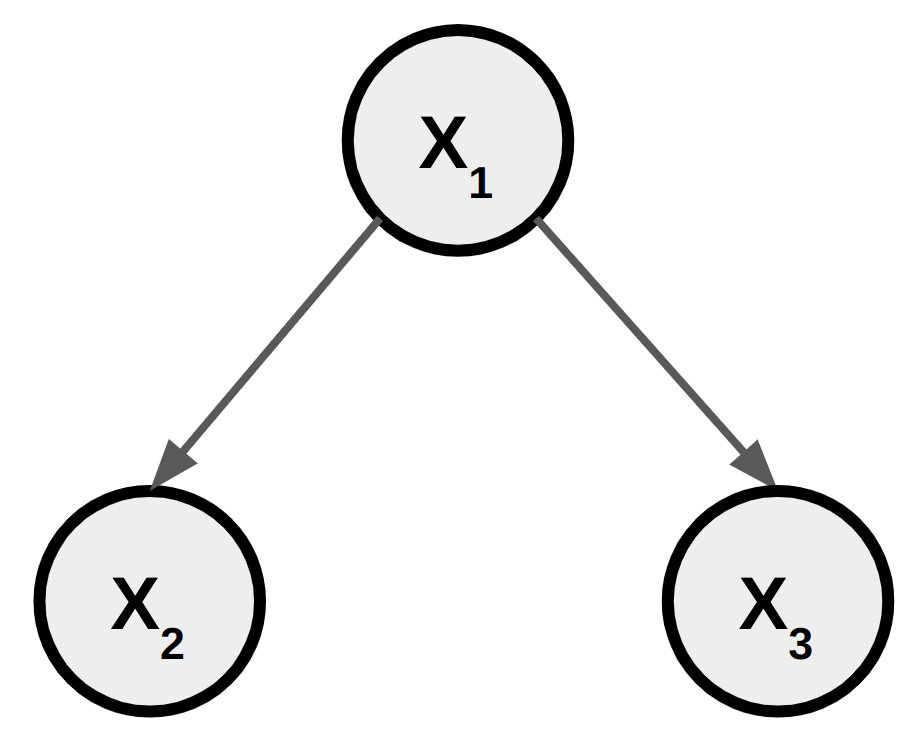
\includegraphics[width=0.5\textwidth]{
		images/10_BayesianNetworksLearning_tailToTailConfiguration.png
	}
	\caption{Three variables linked together with a tail-to-tail configuration.}
	\label{fig:tailToTailLearningBN}
\end{figure}

What is more, we have $N$ examples of this Bayesian network as schematized in
Figure \ref{fig:learningBNExample1}.

\begin{figure}[H]
	\centering
	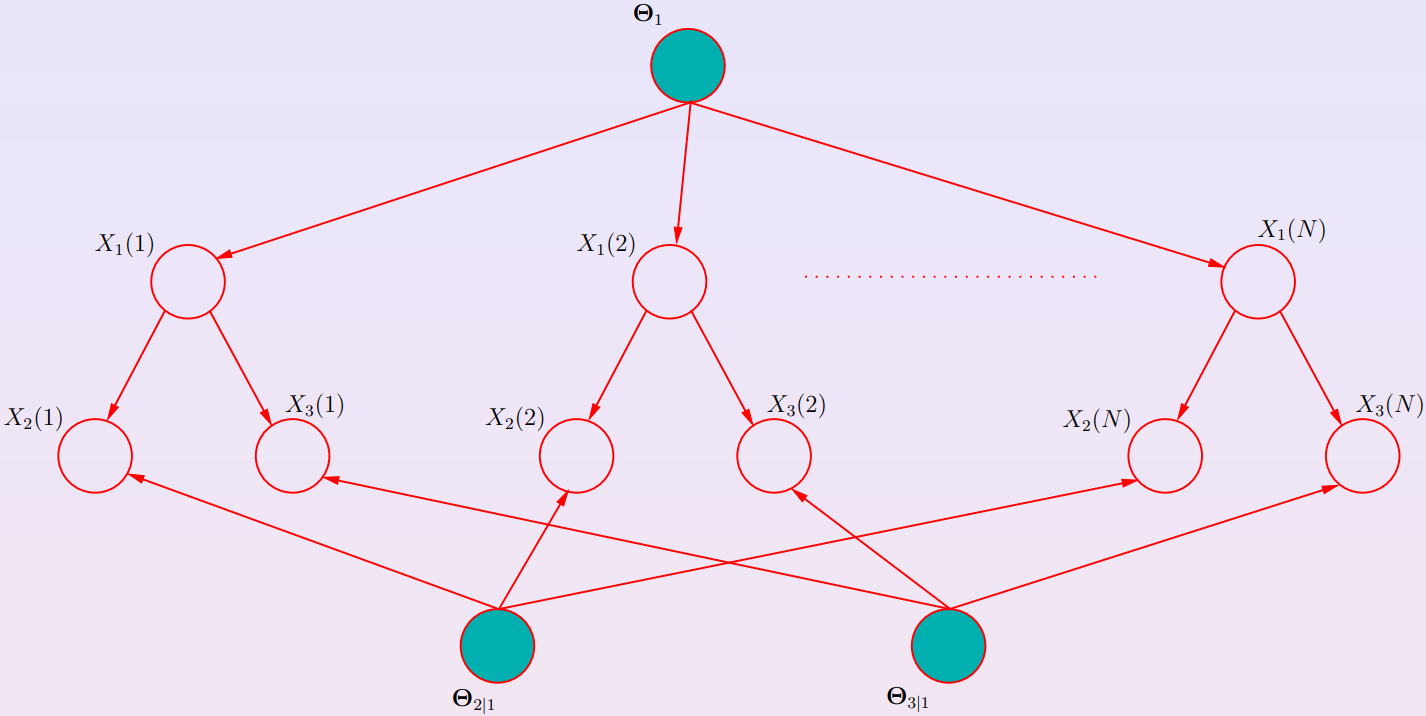
\includegraphics[width=\textwidth]{
		images/10_BayesianNetworksLearning_exampleLearning1.png
	}
	\caption{$N$ examples of the Bayesian network reported in Figure
	\ref{fig:tailToTailLearningBN}.}
	\label{fig:learningBNExample1}
\end{figure}

At this point, our aim is to write down an expression for
$p(\mathcal{D}|\pmb{\theta})$. Since data are iid given the parameters $\pmb{\theta}$,
then we can write:
\[
	p(\mathcal{D}|\pmb{\theta}) = \prod_{i=1}^{N} p(\pmb{x}(i) | \pmb{\theta})
\]
Now, we can go through the factorization of the BN to rewrite
$p(\pmb{x}(i) | \pmb{\theta})$:
\[
	p(\mathcal{D}|\pmb{\theta}) = \prod_{i=1}^{N} \prod_{j=1}^{m} p(\pmb{x}_{j}(i)
	| \mathit{pa}_{j}(i), \pmb{\theta})
\]
Notice that in Figure \ref{fig:learningBNExample1}, we replicate the model $N$
times. Each instance of the BN is related to a different example.\\ When computing
$p(\pmb{x}_{j}(i) | \mathit{pa}_{j}(i))$, this probability depends only on a
subset of the parameters $\pmb{\theta}_{X_j | \mathit{pa}_j}$ which are
interesting (are part of the table) in that particular conditional probability
distribution. So, the probability $p(\pmb{x}_{j}(i) | \mathit{pa}_{j}(i))$
depends only on $\pmb{\theta}_{X_j | \mathit{pa}_j}$ and does not depend on
other parameters in the network.
\begin{equation}
	\label{eq:factorizationLearningBN}p(\mathcal{D}|\pmb{\theta}) = \prod_{i=1}^{N}
	\prod_{j=1}^{m} p(\pmb{x}_{j}(i) | \mathit{pa}_{j}(i), \pmb{\theta}_{X_j |
	\mathit{pa}_j})
\end{equation}
This concept is described graphically in Figure \ref{fig:learningBNExample1} as follows:
\begin{itemize}
	\item $\pmb{\Theta}_{1}$ are the parameters associated to $X_{1}$. Evidently, $X
		_{1}$ is not a conditional probability distribution.

	\item $\pmb{\Theta}_{2|1}$ are the parameters associated to $X_{2}$.

	\item $\pmb{\Theta}_{3|1}$ are the parameters associated to $X_{3}$.
\end{itemize}
It is important to notice that the directional arrows are from the parameters to
the nodes in the network. Indeed, at a high level the structure models
$p(\mathcal{D}|\pmb{\theta}) p(\pmb{\theta})$. So parameters are parents with respect
to the data.
\newline

\textbf{Remark:} If we try to build a Bayesian network which has the
factorization of Equation \ref{eq:factorizationLearningBN} we would recover the
network structure illustrated in Figure \ref{fig:learningBNExample1}. For instance,
suppose we have three nodes $X_{1}$, $X_{2}$, $X_{3}$ and $N=2$ examples. Then from
Equation \ref{eq:factorizationLearningBN} we get:
\begin{align*}
	p(\mathcal{D}|\pmb{\theta}) & = \prod_{i=1}^{N} \prod_{j=1}^{m} p(\pmb{x}_{j}(i) | \mathit{pa}_{j}(i), \pmb{\theta}_{X_j | \mathit{pa}_j}) \\
	                            & = p(X_{1}(1) | \theta_{X_1}) p(X_{2}(1)|X_{1}(1), \theta_{X_2|X_1}) p(X_{3}(1) | X_{1}(1), \theta_{X_3|X_1}) \\
	                            & p(X_{1}(2) | \theta_{X_1}) p(X_{2}(2)|X_{1}(2), \theta_{X_2|X_1}) p(X_{3}(2) | X_{1}(2), \theta_{X_3|X_1})
\end{align*}
Notice that the parameters $\theta_{X_1}, \theta_{X_2|X_1}, \theta_{X_3|X_1}$, do
not depend on the specific example.\\ If we try to draw the corresponding network
we get the model illustrated in Figure \ref{fig:learningBNSmallExample}.

\begin{figure}[H]
	\centering
	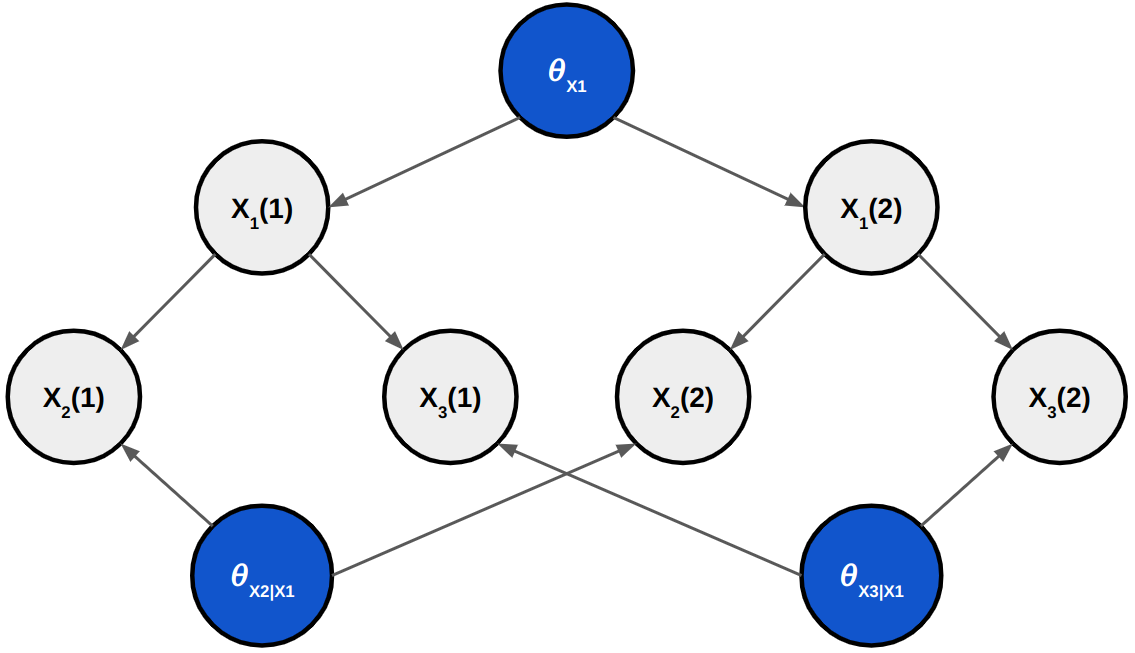
\includegraphics[width=\textwidth]{
		images/10_BayesianNetworksLearning_exampleLearning2.png
	}
	\caption{$N=2$ examples of the Bayesian network reported in Figure
	\ref{fig:tailToTailLearningBN}.}
	\label{fig:learningBNSmallExample}
\end{figure}

\section{Maximum likelihood estimation, complete data}
The parameters of each CPD (conditional probability distribution) can be
estimated independently:
\begin{equation}
	\label{eq:maximum_likelihood_estimation_complete_data}\pmb{\theta}^{\mathit{max}}
	_{X_j | \mathit{pa}_j}= \mathit{argmax}_{\pmb{\theta}_{X_j | \mathit{pa}_j}}\prod
	_{i=1}^{N} p(\pmb{x}_{j}(i) | \mathit{pa}_{j}(i), \pmb{\theta}_{X_j |
	\mathit{pa}_j}) = \mathcal{L}(\pmb{\theta}_{X_j|\mathit{pa}_j}, \mathcal{D})
\end{equation}
In other words, if we want to maximize with respect to
$\pmb{\theta}_{X_j | \mathit{pa}_j}$, we do not take care about other $\pmb{\theta}
_{X_{j'} | \mathit{pa}_{j'}}$ such that $j \neq j'$. Indeed, we are maximizing $\prod
_{i=1}^{N} \prod_{j=1}^{m} p(\pmb{x}_{j}(i) | \mathit{pa}_{j}(i), \pmb{\theta}_{X_j
| \mathit{pa}_j})$ with respect to the parameters related to the $j^{\mathit{TH}}$
node. In the product, everything which is not $j$ is constant with respect to $j$,
as a result we can ignore everything which is not $j$ when maximizing. In Equation
\ref{eq:maximum_likelihood_estimation_complete_data} we remove the product over $j$,
since we concentrate on a particular value of $j$.\\ We have to compute a
maximization of this kind for each node of the network and so for each
conditional probability distribution. A discrete CPD $P(X|\pmb{U})$, can be
represented as a table (an example is reported in Figure \ref{fig:exampleMaximumLikelihoodEstimationCompleteData})
with:
\begin{itemize}
	\item a number of rows equal to the number $\mathit{Val}(X)$ (2 in the case of
		Figure \ref{fig:exampleMaximumLikelihoodEstimationCompleteData}) of configurations
		for $X$

	\item a number of columns equal to the number $\mathit{Val}(\pmb{U})$ (3 in
		the case of Figure \ref{fig:exampleMaximumLikelihoodEstimationCompleteData})
		of configurations for its parents $\pmb{U}$ (one value if there is one
		parent, multiple values if there is more than one parent)

	\item each table entry $\theta_{X|\pmb{u}}$ indicating the probability of a specific
		configuration of $X=x$ and its parents $\pmb{U}=\pmb{u}$
\end{itemize}

Replacing $p(x(i)|\mathit{pa}(i))$ with $\theta_{x(i)|\pmb{u}(i)}$, the local likelihood
of a single CPD becomes:
\begin{align*}
	\mathcal{L}(\pmb{\theta}_{X|\mathit{Pa}}, \mathcal{D}) & =                                                                                                            \\
	                                                       & = \prod_{i=1}^{N} p(x(i)|\mathit{pa}(i), \pmb{\theta}_{X|\mathit{Pa}})                                      & = \\
	                                                       & = \prod_{i=1}^{N} \theta_{x(i)|\pmb{u}(i)}                                                                  & = \\
	                                                       & = \prod_{\pmb{u} \in \mathit{Val}(\pmb{U})}[\prod_{x \in \mathit{Val}(X)}\theta^{N_{\pmb{u},x}}_{x|\pmb{u}}]
\end{align*}
where $N_{\pmb{u},x}$ is the number of times the specific configuration $X=x$, $\pmb
{U}=\pmb{u}$ was found in the data.
\newline

\textbf{Remark:} in principle we should keep the $j$ index. However, we omit it
since node $j$ is independent with respect to all other nodes. As a result we can
present results for a generic node. Following this approach, each node is treated
independently.
\newline

\begin{figure}[H]
	\centering
	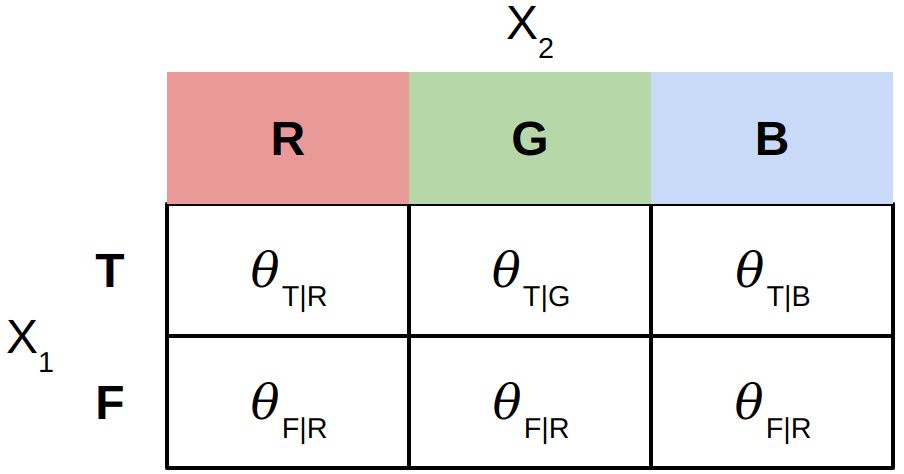
\includegraphics[width=0.8\textwidth]{
		images/10_BayesianNetworksLearning_discreteDistributionTable.png
	}
	\caption{A discrete CPD represented as a table.}
	\label{fig:exampleMaximumLikelihoodEstimationCompleteData}
\end{figure}

In essence, for all possible parameter in the conditional probability distribution,
the likelihood becomes
$\mathit{parameter}^{\mathit{number of times I see that configuration in my
dataset}}$
\newline

A column in the CPD table contains a multinomial distribution over values of $X$
for a certain configuration of the parents $\pmb{U}$. Thus, each column should sum
to one:
\[
	\sum_{x} \theta_{x|\pmb{u}}=1
\]
Parameters of different columns can be estimated independently. For each multinomial
distribution, zeroing the gradient of the maximum likelihood and considering the
normalization constraint, we obtain:
\[
	\theta^{\mathit{max}}_{x|\pmb{u}}= \frac{\pmb{N}_{\pmb{u},x}}{\sum_{x} \pmb{N}_{\pmb{u},x}}
\]
At the end of the day, the maximum likelihood parameters are simply the fraction
of times in which the specific configuration was observed in the data.
\newline

\textbf{Example}
\newline
In this example we consider the situation illustrated in Figure
\ref{fig:exampleMaximumLikelihoodEstimationCompleteData}. Suppose that our dataset
is populated as follows:
\begin{center}
	\begin{tabular}{ |c|c|c| }
		$X_{1}$ & $X_{2}$ & $X_{3}$ \\
		\hline
		T       & R       & F       \\
		T       & R       & F       \\
		T       & G       & T       \\
		F       & R       & F       \\
		T       & B       & T       \\
		T       & B       & T       \\
		T       & B       & T       \\
	\end{tabular}
\end{center}
In this case the likelihood function which we want to maximize becomes:
\begin{equation}
	\label{eq:exampleTableMaximumLECompleteData}\mathcal{L}(\pmb{\theta}_{X|\mathit{Pa}}
	, \mathcal{D}) = \theta^{2}_{T|R}\theta_{T|G}\theta^{3}_{T|B}\theta_{F|R}
\end{equation}
Remember that the columns in the table must sum to one. As a consequence, the purpose
of the problem is to maximize Equation \ref{eq:exampleTableMaximumLECompleteData}
subject to the fact that the columns in the table sum to one. As a result, there
are no connections among columns. So, in \ref{eq:exampleTableMaximumLECompleteData}
we consider $\theta^{2}_{T|R}$ and $\theta_{F|R}$ together because they have to sum
to one. On the other hand, for $\theta_{T|G}$ and $\theta^{3}_{T|B}$ we have no constraints
with respect to the other variables in the formula, so we can maximize them
independently. In essence, in the maximization, each column (i.e. a configuration
for the parents) can be treated independently. Maximizing a single column means maximizing
over a single distribution which corresponds to the column. So, we face the maximization
problem, dividing it into pieces until we end up maximizing individual
distributions. \\ In this case:
\begin{equation}
	\label{eq:parameterMaximizationGraphicalModel}\theta^{\mathit{max}}_{x|\pmb{u}}
	= \frac{\pmb{N}_{\pmb{u},x}}{\sum_{x} \pmb{N}_{\pmb{u},x}}
\end{equation}
\begin{itemize}
	\item $\theta_{T|R}= \frac{2}{3}$

	\item $\theta_{T|G}= \frac{1}{1}$

	\item $\theta_{T|B}= \frac{3}{3}$

	\item $\theta_{F|R}= \frac{1}{3}$

	\item $\theta_{F|G}= 0$

	\item $\theta_{F|B}= 0$
\end{itemize}

\textbf{Remark:} this is a toy example. In real world scenarios, it is not ideal
to have probability 1 or probability 0. For example, if the estimation of a probability
is zero it nullify the joint probability of the whole network. In order to deal
with this problem, we introduce priors.

\subsection{Adding priors}
Maximum likelihood estimation tends to overfit the training set. Configuration
not appearing in the training set will receive zero probability. A common approach
consists of combining maximum likelihood with a prior probability on the parameters,
achieving a maximum-a-posteriori estimate:
\begin{equation}
	\pmb{\theta}^{\mathit{max}}= \mathit{argmax}_{\pmb{\theta}}p(\mathcal{D}|\pmb{\theta}
	)p(\pmb{\theta})
\end{equation}
In this case, our aim is to compute the configuration
$\pmb{\theta}^{\mathit{max}}$ which maximizes not the likelihood but the
posterior.
\newline

\textbf{Remark:} the posterior is $p(\pmb{\theta}|\mathcal{D})$:
\[
	p(\pmb{\theta}|\mathcal{D}) = \frac{p(\mathcal{D}|\pmb{\theta}) p(\pmb{\theta})}{p(\mathcal{D})}
\]
$p(\mathcal{D})$ does not depend on $\pmb{\theta}$. So, maximizing
$p(\pmb{\theta}|\mathcal{D})$ is the same as maximizing
$p(\mathcal{D}|\pmb{\theta})p(\pmb{\theta})$ since $p(\mathcal{D})$ is constant
($p(\pmb{\theta}|\mathcal{D}) \propto p(\mathcal{D}|\pmb{\theta}) p(\pmb{\theta})$).
\newline

The conjugate (read natural) prior for a multinomial distribution is a Dirichlet
distribution with parameters $\alpha_{x|\pmb{u}}$ for each possible value of $x$.
The resulting maximum-a-posteriori estimate is:
\begin{equation}
	\theta^{\mathit{max}}_{x|\pmb{u}}= \frac{\pmb{N}_{\pmb{u},x}+ \alpha_{x|\pmb{u}}}{\sum_{x}
	(\pmb{N}_{\pmb{u},x}+ \alpha_{x|\pmb{u}})}
\end{equation}
The prior is like having observed $\alpha_{x|\pmb{u}}$ imaginary samples with
configuration $X=x$, $\pmb{U}=\pmb{u}$. \\ For example, we could assume to have seen
each configuration 1 (or a fraction of 1) times by coherently setting each $\alpha
_{x|\pmb{u}}$. In this way we avoid to get zero probabilities.

\section{Maximum likelihood estimation, incomplete data}
Up to this point we have considered only complete data such that, for each example
we have fully observed data (we know the value for every variable). With
incomplete data, some of the examples miss evidence on some of the variables.
Counts of occurrences of different configurations cannot be computed if not all
data are observed. The full Bayesian approach of integrating (in the discrete
case, sum up) over missing variables is often intractable in practice. We need approximate
methods to deal with the problem.
\newline

\textbf{Example:} for example we could have question marks for some
configurations:
\begin{center}
	\begin{tabular}{ |c|c|c| }
		$X_{1}$ & $X_{2}$ & $X_{3}$ \\
		\hline
		T       & R       & F       \\
		?       & R       & F       \\
		T       & G       & T       \\
		F       & ?       & F       \\
		T       & B       & T       \\
		T       & ?       & T       \\
		T       & B       & T       \\
	\end{tabular}
\end{center}
This is the case of the medical domain where it is unlikely that a person does all
the possible exams. This of course results in a lot of missing data.
\newline

The idea is to take advantage of the graphical model in order to compute the
probability of what we do not know given what we know. For instance, in the
context of the table above, we could use the graphical model to compute $P(X_{1}=
T | X_{2}=R, X_{3}=F)$. This latter becomes a replacement for the corresponding
entry of the table. The question mark is replaced by a probability of being true
or false. \\ However, in order to compute the probability $P(X_{1}=T | X_{2}=R, X
_{3}=F)$ we need the parameters $\theta_{T|R}, \theta_{T|G}, \theta_{T|B},\theta_{F|R}
, \theta_{F|G}, \theta_{F|B}$ which we are trying to estimate. This chicken and
egg problem is solved using an iterative procedure. This last is called \textit{Expectation-Maximization}.

\subsection{Expectation-Maximization}
Sufficient statistics (counts) cannot be computed due to missing data. Remember that
the counts are the sufficient statistics, i.e. all we need of the data. At the
beginning we can initialize the parameters in some ways as we discuss in the
following. After that, we fill-in missing data inferring them using current
parameters by solving inference problem to get expected counts. In other words,
we compute the probability of a certain configuration given the current
parameters and what we already know (the non-missing data). Using these probabilities
we can compute the so called \textit{expected counts}. These lasts are named "expected"
since we do not have certain values for some variables. Then, we compute parameters
maximizing likelihood (or posterior) of such expected counts (using the expected
counts as if they are the exact counts). Finally, we iterate the procedure to improve
the quality of the parameters. Indeed, with the updated parameters we can re-compute
the expected counts. The procedure is iterated until nothing changes anymore (i.e.
there is no parameters update). This procedure is guaranteed to converge to a
local maximum of the likelihood. The quality of this local optimum depends significantly
on the initial point which is the initial configuration of the parameters.

\subsection{Expectation-Maximization algorithm: e-step}
Our aim is to compute the expected sufficient statistics (i.e. the expected counts)
for the complete dataset, with expectation taken with respect to the joint distribution
for $\pmb{X}$ ($\pmb{X}_{l}$ is what I know about the $l^{\mathit{TH}}$ example,
i.e. the evidence) conditioned of the current value of $\pmb{\theta}$ (current
estimate of the parameter) and the known data $\mathcal{D}$:
\begin{equation}
	E_{p(\pmb{X}|\mathcal{D}, \pmb{\theta})}[N_{ijk}] = \sum_{l=1}^{n} p(X_{i}(l) =
	x_{k}, \mathit{Pa}_{i}(l) = \mathit{pa}_{j} | \pmb{X}_{l}, \pmb{\theta})
\end{equation}
\begin{itemize}
	\item In the formula $N_{ijk}$ is the count for the configuration where example
		$X_{i}$ takes value $x_{k}$ and the parents $\mathit{Pa}_{i}$ of the example
		$X_{i}$ takes value $\mathit{pa}_{j}$. So, $i$ is the node in the network,
		$k$ is the value for that node, $j$ is the value of the parent. $i$
		identifies the table, $j$ and $k$ identify the entry of the table.

	\item If $X_{i}(l)$ and $\mathit{Pa}_{i}(l)$ are observed for $\pmb{X}_{l}$,
		it is either zero or one. (In the case of complete data, for each example we
		check if the particular configuration holds for that example and we sum up obtaining
		an integer which is the real count).

	\item Otherwise, run Bayesian inference to compute probabilities from observed
		variables. ($\sum_{l=1}^{n}$ is the sum over the set of examples) ($X_{i}(l)$
		represents node $i$ in the $l^{\mathit{TH}}$ example) ($\mathit{Pa}_{i}(l)$
		represents the parent of node $i$ in the $l^{\mathit{TH}}$ example)
\end{itemize}

This step is called \textit{expectation step} (e-step).

\subsection{Expectation-Maximization algorithm: m-step}
The second step is called \textit{maximization step} (m-step). The purpose of
this step is to compute parameters maximizing the likelihood of the complete
dataset $D_{c}$ using the expected counts.
\begin{equation}
	\pmb{\theta}^{*} = \mathit{argmax}_{\pmb{\theta}}p(D_{c}|\pmb{\theta})
\end{equation}
In the formula, $D_{c}$ represents the dataset filled with the expected counts. For
each multinomial parameter $\theta^{*}_{ijk}$ evaluates to:
\begin{equation}
	\theta^{*}_{ijk}= \frac{E_{p(\pmb{X}|\mathcal{D}, \pmb{\theta})}[N_{ijk}]}{\sum_{k=1}^{r_i}E_{p(\pmb{X}|\mathcal{D},
	\pmb{\theta})}[N_{ijk}]}
\end{equation}
Actually, this is an extension of Equation \ref{eq:parameterMaximizationGraphicalModel}
using expected counts instead of actual counts.
\newline

\textbf{Remark:} maximum likelihood estimation can be replaced by maximum a-posteriori
(MAP) estimation giving:
\begin{equation}
	\theta^{*}_{ijk}= \frac{\alpha_{ijk}+ E_{p(\pmb{X}|\mathcal{D}, \pmb{\theta})}[N_{ijk}]}{\sum_{k=1}^{r_i}(\alpha_{ijk}+E_{p(\pmb{X}|\mathcal{D},
	\pmb{\theta})}[N_{ijk}])}
\end{equation}

At the end of this step, we get a new estimate of the parameters $\pmb{\theta}$.
We iteratively execute the e-step with the updated parameter estimation. The iterative
procedure proceeds in this manner until convergence.

\section{Learning structure of graphical models}
So far, we have assumed that the structure of the network is given (and we try to
learn the parameters). However, this is not always the case of course. If we have
domain knowledge we could try to construct the graphical model. However, this is
not always possible. Typically, we know some relationships, but we do not know
everything. In order to face this problem, the literature suggests three main
approaches:

\begin{itemize}
	\item \textbf{Constraint-based:} test conditional independencies on the data
		and construct a model satisfying them. With this approach we rely on hypothesis
		testing techniques to verify dependency or independency between pairs of variables.
		Then based on the result of these tests, we add connections to the network.
		Typically this method does not allow to learn the directions of the
		connections.

	\item \textbf{Score-based:} assign a (probabilistic) score to each possible
		structure, define a search procedure looking for the structure maximizing the
		score. With this approach we move in the space of possible structures guided
		by the score.

	\item \textbf{Model-averaging:} given that we do not know the network
		structure, we treat it as a random variable. We assign a prior probability
		to each structure, and average prediction over all possible structures weighed
		by their probabilities (full Bayesian, intractable since the number of possible
		structures is exponential with respect to the number of variables). This approach
		is a kind of ensemble learning method where we generate more than one structure
		and average the prediction in a similar way as we have seen for random forests.
		This could increase the robustness of the predictions but leads often to
		less explainable results.
\end{itemize}